%XeLaTeX
\documentclass{article}
\usepackage{lscape}
\usepackage{fontspec}
\setmainfont{DejaVu Serif}
\newfontfamily{\tam}[Script=Tamil]{NotoSerifTamilSlanted-Regular}
%\newfontfamily{\tam}[Script=Tamil]{FreeSerif}
\defaultfontfeatures{Scale=MatchLowercase}
\usepackage[dvipsnames]{xcolor}
\usepackage{eso-pic,graphicx}
\usepackage[top=51mm, bottom=51mm, outer=80mm, inner=80mm, landscape]{geometry}
\usepackage{graphicx}
\graphicspath{ {./ } }
\usepackage[figurename=]{caption}
\usepackage{float}
\color{White}
\AddToShipoutPictureBG{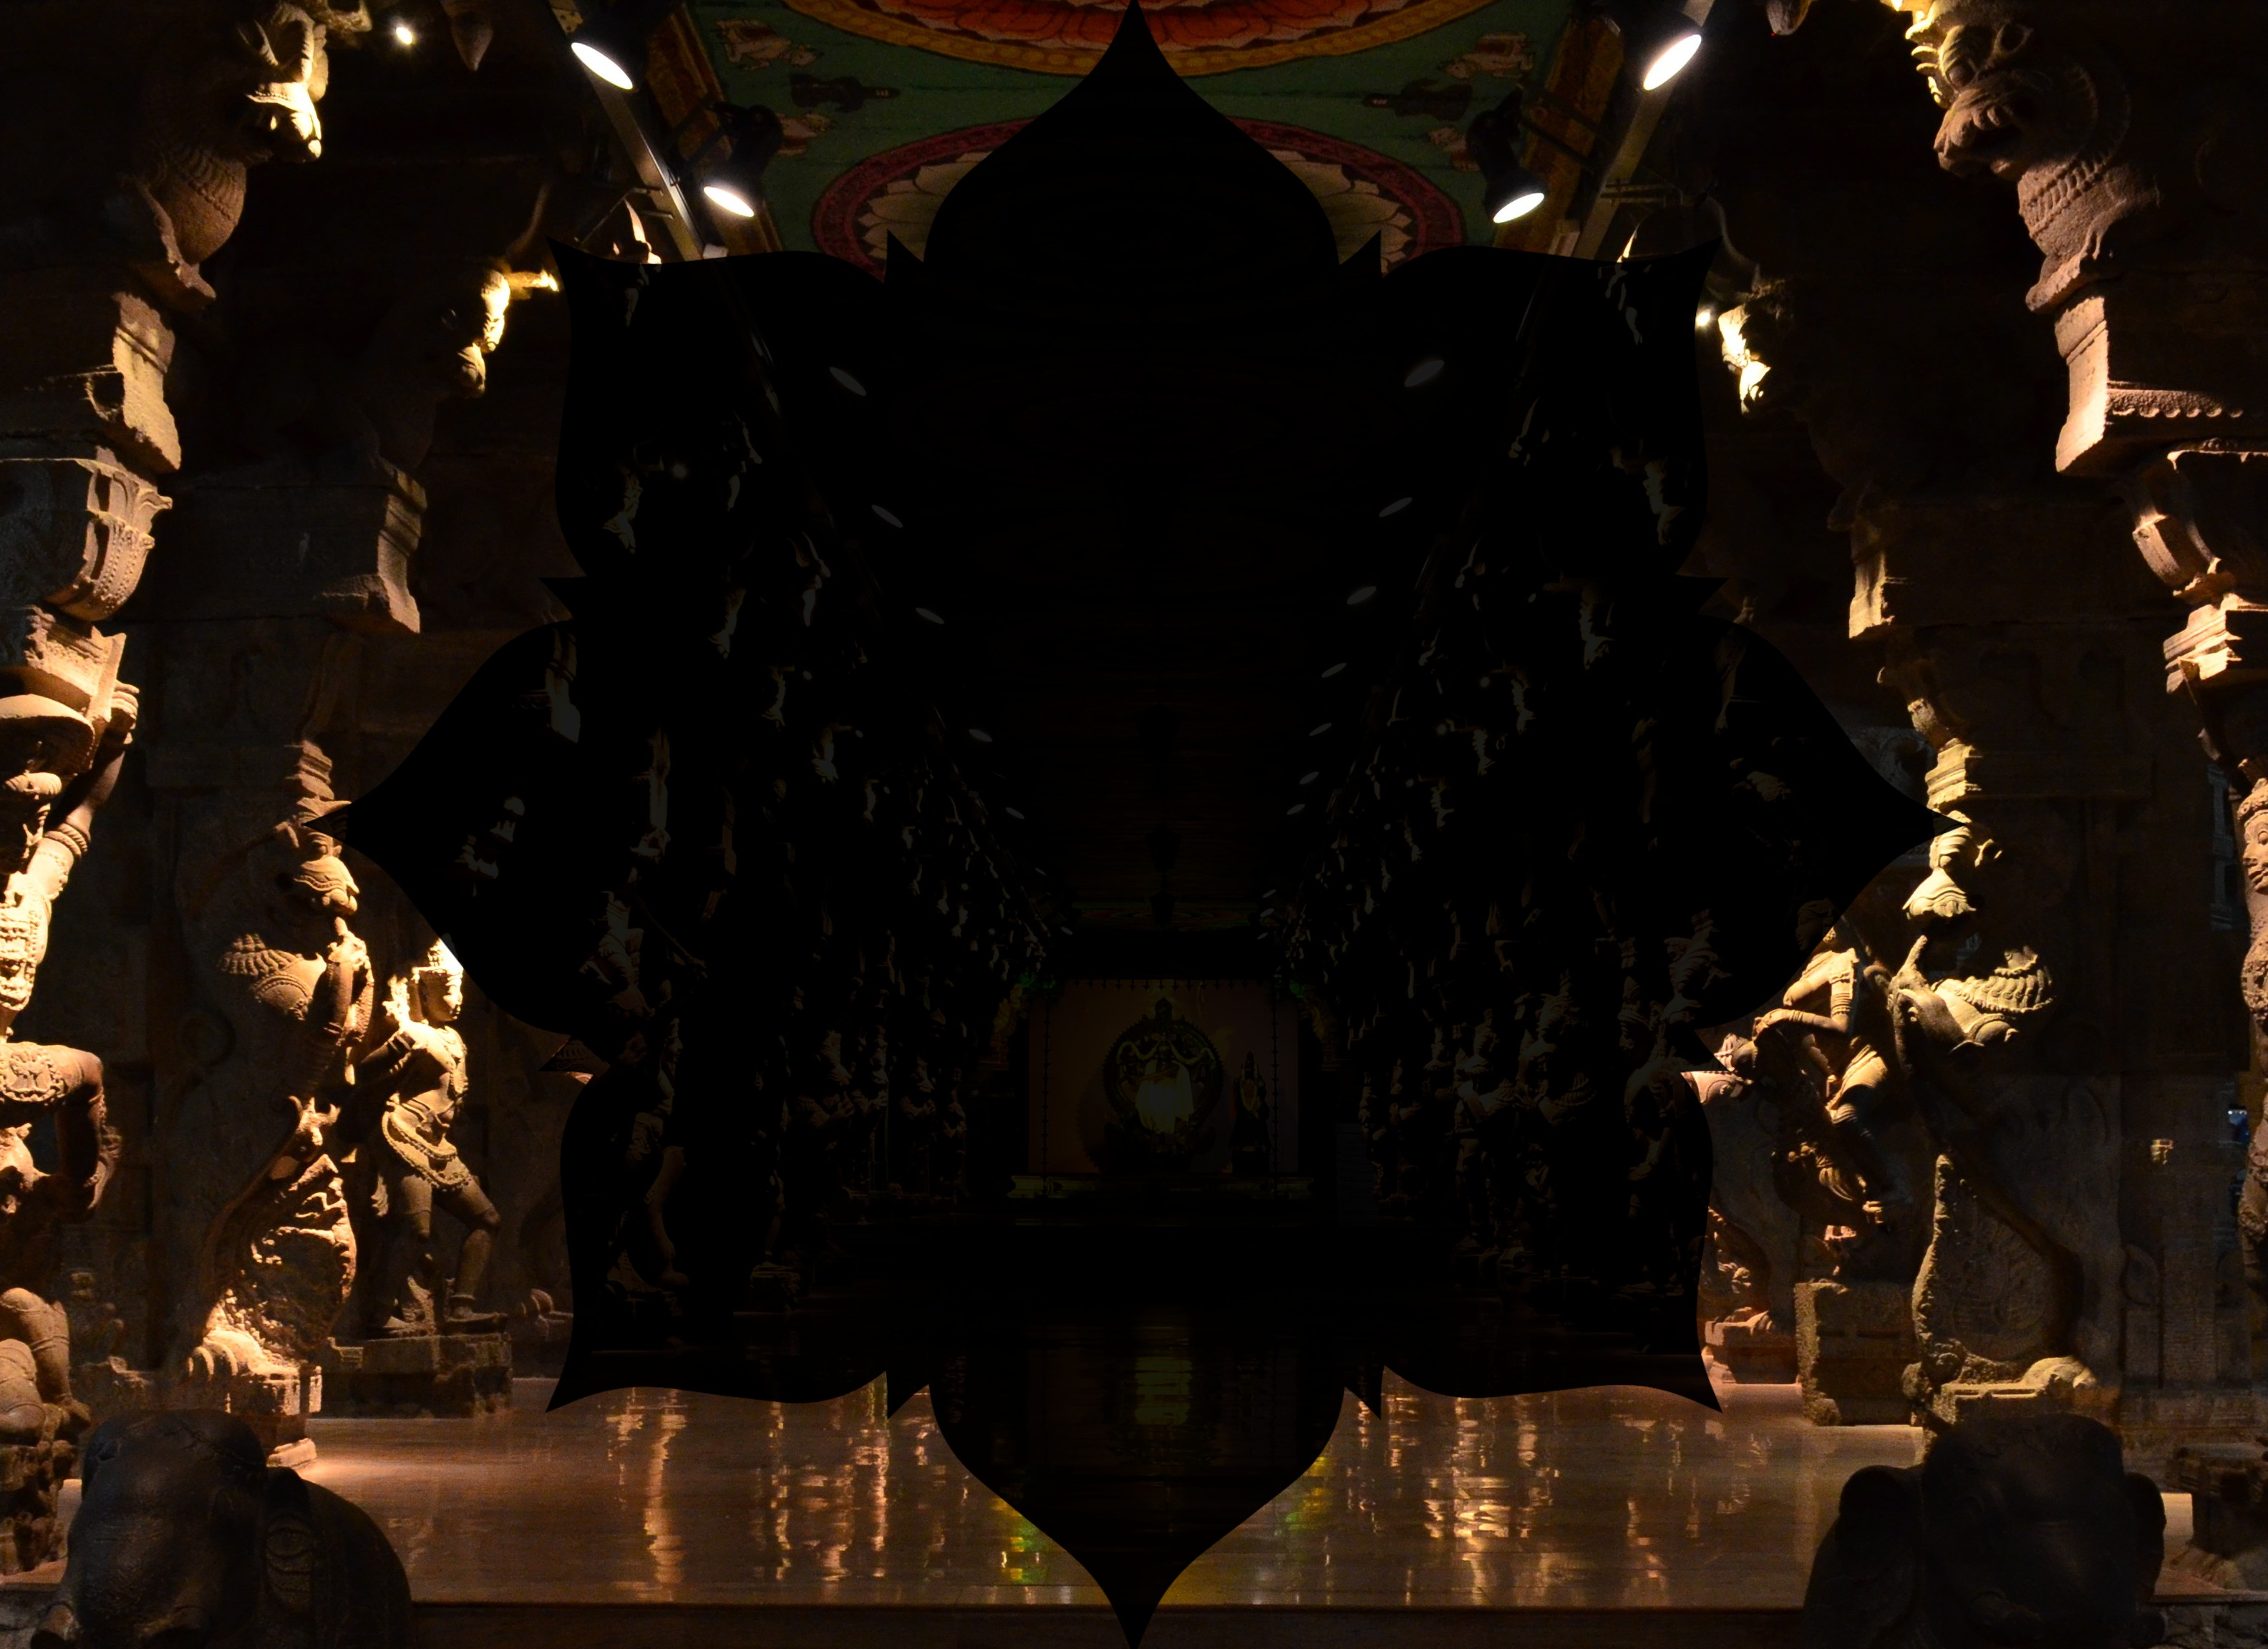
\includegraphics[width=\paperwidth,height=\paperheight]{amma1.jpeg}}
\begin{document}
\begin{titlepage} % Suppresses headers and footers on the title page
	\centering % Centre everything on the title page
	%\scshape % Use small caps for all text on the title page

	%------------------------------------------------
	%	Title
	%------------------------------------------------

	\rule{\textwidth}{1.6pt}\vspace*{-\baselineskip}\vspace*{2pt} % Thick horizontal rule
	\rule{\textwidth}{0.4pt} % Thin horizontal rule
	
	\vspace{1\baselineskip} % Whitespace above the title
	
	{\scshape\Huge \tam{மாரியமஂமனஂ தாலாடஂடு}}
	
	\vspace{1\baselineskip} % Whitespace above the title

	\rule{\textwidth}{0.4pt}\vspace*{-\baselineskip}\vspace{3.2pt} % Thin horizontal rule
	\rule{\textwidth}{1.6pt} % Thick horizontal rule
	
	\vspace{1\baselineskip} % Whitespace after the title block
	
	%------------------------------------------------
	%	Subtitle
	%------------------------------------------------
	
        {\small \tam{௳}\\\tam{சடவுள்‌ தணை}}
 
        \vspace{1.0\baselineskip}
		
        {\scriptsize \tam{எத்தேசங்களிலும்‌ இடைவிடாமற் சிந்‌தித்துவரும்‌‌.}\\\tam{இ ன வ}\\\Large\tam{பூவிருந்தவல்லி, தங்கவேலுமுதலியா ரவா்களால்‌, பரா்வையிடப்பட்டு}} % Subtitle or further description

        \vspace{1.0\baselineskip}

        {\small \tam{சென்னை-சூளை}\\\tam{பு. மூனிசாமிநாயுடு}\\\tam{அவா்களசி}\\\tam{சங்ககிதிவிளக்க ௮ச்சுச்கூடத்திற்}}
‌
	%------------------------------------------------
	%	Editor(s)
	%------------------------------------------------
        \vspace*{\fill}    

	\vspace{1\baselineskip}

        {\small\tam{பதிப்பிக்கப்பட்டசி}, 1920}
		
	\vspace{0.25\baselineskip} % Whitespace after the title block

        {\scshape\small Internet Archive Online Edition}% Publication year}
    
	{\scshape\footnotesize Attribution NonCommercial ShareAlike 4.0 International } % Publisher
\end{titlepage}
\clearpage
\vspace*{\fill}  
\begin{figure}[H]
\centering
\includegraphics[width=0.75\textwidth,keepaspectratio]{white/fig001.png}
\end{figure}
\vspace*{\fill}  
\clearpage
\begin{figure}[H]
\centering
\includegraphics[width=0.95\textwidth,keepaspectratio]{white/fig006.png}
\end{figure}
\begin{center}
\tam{

௳

பராசத்தி அனை.

எத்தேசங்களிலும்‌ இடைவிடாமற் சிந்தித்துவரும்.
}

\bigskip

{\Large\tam{மாரியமஂமனஂ தாலாடஂடு.}}
\end{center}
\begin{figure}[H]
\centering
\includegraphics[width=0.5\textwidth,keepaspectratio]{white/fig007.png}
\end{figure}
\begin{center}
\tam{

விநாயகா் துதி.

காப்பு.

சொச்சக்கலிப்பா.
}
\end{center}
\begin{quotation}
\tam{
பூசலத்தில்‌ யாவா்களும்‌ போதரவா யென்னாளும்

மாதரசி யென் று வாழ்த்துகின்ற மாரியம்மன்

சீதரனா் தங்கைச்‌ சிறப்பான தாலாட்டைக்

காதலுட னேதக் கணபதியுங் காப்பாமே.
}
\end{quotation}
\begin{figure}[H]
\centering
\includegraphics[width=0.9\textwidth,keepaspectratio]{white/fig002.png}
\caption*{\tam{வெண்செந்துறை.}}
\end{figure}
\begin{quotation}
\tam{\small 
முந்திமுந்திவிசாயகரே முக்கணனா்தன்மகனே

சந்தருக்குமுன்பிறச்த சற்பகமேமுன்னடவாய்‌

வேலவர்க்குமுன்பிறந்த விநாயகரேமுன்னடவாய்‌‌

வேம்படியிற்பிள்ளையாரே விக்கினரேமுன்னடவாய்

‌
பேழைவயிற்றோனே பெருச்சாளிவாகனரே

காராணமால்மருகா கற்பகமேமெய்ப்பொருளே

சீரானநல்மருகா செல்வக்கணபதியே

ஒற்றைக்கொம்போனே உமையாள்‌திருமகனே

கற்றைச்சடையணிந்த கங்காதரன்மகனே

வித்தைக்குவிநாயகனே வெண்ணையுண்டோன்மருகா

மத்தக்கரிமுகவா மாயோன்மருகோனே

ஐந்துகரத்தோனே யானைமுகத்தோனே

தந்திமதவாரணனே தற்பரனேமுன்னடவாய்‌

நெஞ்சிற்குடியிருந்‌து நீயெனக்குமுன்னடவாய்

‌
பஞ்சஞ்சுமெல்லடியாள்‌ பார்வதியாள்புத்‌திரனே

வேழமுகத்தோனே விநாயகரேமுன்னடவாய்‌

தாழ்வில்லாச்சங்கரனார் சற்புத்திராவாருமையா

முன்னடக்கும்பிள்ளையார்க்குக்‌ கண்ணடக்கம்பொன்னாலே

கண்ணடக்கம்பொன்னாலே காற்சிலம்புமுத்தாலே

முத்தாலேதண்டைகொஞ்ச முன்னடவாய்பிள்ளையாரே

செல்வக்கணபதியுன் சீர்பாதம்நான்மறவேன்.
}
\end{quotation}
\begin{figure}[H]
\centering
\includegraphics[width=0.9\textwidth,keepaspectratio]{white/fig003.png}
\caption*{\tam{சரஸ்வதி துதி.}}
\end{figure}
\begin{quotation}
\tam{\small 
தாயேசரஸ்வதியே சங்கரியேமுன்னடவாய்

என்தாயேகலைவாணி ஏகவல்லிநாயகியே

வாணிசரஸ்வதியே வாக்கில்குடியிருந்து

என்னாவிற்குடியிருந்து நல்லோசைதாருமம்மா

கமலாசனத்தாளே காரடிபெற்றவளே

என்-குரலிற்குடியிருந்து கொஞ்சடிபெற்றவளே

என்னாவுதவறாமல் நல்லோசைாருமம்மா

மாரியம்மன்தன்கதையை மனமகிழ்ந்துநான்பாட

சரியாகயென்னாவில் தங்கிக்குடியிரம்மா

கன்னனூர்மாரிமுத்தே கைதொழுதுநான்பாட

பின்னமில்லாமற் பீறகிருந்துகாருமம்மா
}
\end{quotation}
\begin{figure}[H]
\centering
\includegraphics[width=0.9\textwidth,keepaspectratio]{white/fig004.png}
\caption*{\tam{மாரியம்மன் துதி.}}
\end{figure}
\begin{quotation}
\tam{\small 
மாயிமகமாயி மணிமந்திரசேகரியே

ஆயிவுமையவளே ஆதிசிவன்தேவியரே

மாரித்தாய்வல்லவியே மகாராசிவாருமம்மா

மாயன்சகோதரியே மாரிமுத்தேவாருமம்மா

ஆயன்சகோதரியே ஆஸ்தானமாரிமுத்தே

தாயேதுரந்தரியே சங்கரியேவாருமம்மா

திக்கெல்லாம்போற்று மெக்கலாதேவியரே

எக்கலாதேவியரே திக்கெல்லாம்நின்றசக்தி

கன்னபுரத்தாளே காரணசவுந்தரியே

காரணசவுந்தரியே நாரணனார்தங்கையம்மாள்

நாரணனார்தங்கையம்மாள் நல்லமுத்துமாரியரே

உன்-கரகம்பிறந்ததம்மா கஊ்னனூர்மேடையிலே

உன்-வேம்புபிறந்ததம்மா விஜயநகர்பட்டணமாம்

உன்-சூலம்பிறந்ததம்மா துலங்குமணிமண்டபத்தில்

உன்-அலகுபிறந்ததம்மா அயோத்திநகர்பட்டணமாம்

உன்-பிரம்புபிறந்ததம்மா பிச்சாண்டிசந்நிதியாம்

உன்-உடுக்கைபிறந்ததம்மா உருத்திராட்சபூமியிலே

உன்-பம்பைபிறந்ததம்மா பளிங்குமாமண்டபத்தில்

உன்-கருத்துப்பிறந்ததம்மா கஞ்சகிரியிந்திரபுரம்

உன்-மருளர்தழைக்கவம்மா வையகங்களீடேற

உன்-குமாரவர்க்கந்தான்றழைக்க கொம்பனையேமாரிமுத்தே
}
\end{quotation}
\begin{figure}[H]
\centering
\includegraphics[height=0.45\textheight,keepaspectratio]{white/fig005.png}
\end{figure}
\begin{quotation}
\tam{\small 
உனக்கு-மூன்றுகரகமம்மா மு்த்தான நற்கரகம்

உனக்கு-ஐந்துகரகமம்மா அசைந்தாடும்பொற்கரகம்

உனக்கு-ஏழுகரகமம்மா எடுத்தாடும்பொற்கரகம்

உனக்கு-பத்துகரகமம்மா பதிந்தாடும்பொற்கரகம்

வேப்பிலையும்பொற்கரகம் வீதிவிளையாடிவர

ஆயிரங்கண்ணுடையாள் அலங்காரிவாருமம்மா

பதினாயிரங்கண்ணுடையாள் பராசக்திவாருமம்மா

துலுக்காணதெல்லையெல்லாம் குலுக்காடப்பெண்பிறந்தாய்

துலுக்கானதெல்லைவிட்டு துரந்தரியேவாருமம்மா

தாயேதுரந்தரியேசங்கரியேவாருமம்மா

மலையாளதேசமெல்லாம் விளையாடப்பெண்பிறந்தாய்

மலையாளதேசவிட்டு வாருமம்மாயிந்தமுகம்

சமைந்தாய்சமையபுரம் சாதித்தா்ய்கன்னபுரம்

இருந்தாய்விலாடபுரம் இனியிருந்தாய்கன்னபுரம்

சமையபுரத்தாளே சாம்பிராணிவாசகியே

சமையபுரத்தெல்லைவிட்டு தாயாரேவாருமம்மா

கன்னபுரத்தாளே காரணசவுந்தரியே

கன்னபுரத்தெல்லைவிட்டு காரணியேவந்தமரும்

கடும்பாடியெல்லையெல்லாங் காவல்கொண்டமாரிமுத்தே

ஊத்துக்காட்டமர்ந்தவளே உதிாபஎிகொண்டவளே

படவேட்டமா்ர்தயளே பாகராமனைப்பெற்றயளே

படவேட்டைவிட்டுமெள்ள பத்தினிபேவாருமம்மா

பெரியபாளையத்தமர்ந்த பேச்சியெனுமாரியரே

பெரியபாளையத்தைவிட்டு பேராசிவாருமம்மா

ஆரணிபெரியபாளையம்மா அதிலிருக்குமாற்றங்கரை

ஆற்றங்கரைமேடைவிட்டு ஆச்சியரேவாருமம்மா

வீராம்பட்டணமமர்நத வேதாந்தமாரிமுததே

கோலியனூரெல்லையிலே குதிகொண்டமாரியரே

அந்தரத்திற்றேரோட அருகேசெடிலசைய

உச்சியிற்றேரோட உயர்ந்தசெடிலசைய

மச்சியிற்றேரோட மகரச்செடிலசைய

பக்கங்கயிரோட பகரச்செடிலசைய

ஆண்டகுருதேசியரை அறியாதமானிடரை

தூண்டிலிட்ஆெட்டிவைக்கத்தோன்றினாய் நீயொருத்தி

சத்தியாய்நீயமர்ந்தாய் தனிக்குட்டிகாவுகொண்டாய்

எல்லையிலேநீயமர்நதாய் எருமைக்கிடாகாவுகொண்டாய்

உன்னைப்போல்தெய்வம் உலகததில்கண்டதில்லை

என்னைப்போல்பிள்ளைகள்தா னெங்குமுண்டுவையகத்தில்

கோர்த்தமுத்துவடமசைய கொங்கைரெண்டும்பாலொழுக

ஏற்றவர்க்குவரந்தருவாய் எக்கலாதேவியரே

எக்கலாதேவியரே திக்கெல்லாமாண்டவளே

திக்கெல்லாமாண்டவளே திகம்பரியேவாருமம்மா

முக்கோணசக்கரத்தில் முதன்மையாய்நின்றசத்தி

அக்கோணந்தன்னில்வந்து ஆச்சியரேவந்தமரும்

தாயேதுரந்தரியே சங்கரியேவாருமம்மா

மாயிமருளியரே மணிமந்திரசேகரியே

வல்லாண்மைக்காரியரே வழக்காடும்மாரிமுத்தே

வல்லவரைக்கொன்றாய் வலியவரைமார்பிளந்தாய்

நீலிகபாலியம்மா நிறைந்ததிருச்சூலியரே

நாலுமூலையோமகுண்டம் நடுவேகனகசபை

கனகசபைவீற்றிருக்கும் காரணசவுந்தரியே

நாரணனார்தங்கையரே நலலமுத்துமாரியரே

நடலைச்சுடலையம்மா நடுச்சுடலைத்தில்லைவனம்

தில்லைவனத்தெல்லைவிட்டு திரும்புமம்மாயிந்தமுகம்

வார்ப்புச்சிலையாளே வச்சிரமணிததேராளே

தூண்டித்துடைபெருமன் தூண்டிமுள்ளுகைபெருமன்

மண்டையிலேதைத்தமுள்ளு மார்புருகிப்போகுதம்மா

பக்கத்திற்றைத்தமுள்ளு பதைத்துத்துடிக்குதம்மா

தொண்டையிலேதைததமுள்ளு தோளுருவிப்போகுதம்மா

கத்திப்போல்வேப்பிலையைக் கதறவிட்டாய்லோகமெல்லாம்

ஈட்டிப்போல்வேப்பிலையை யினியனுப்பிக்கொண்டவளே

பத்திரிக்குள்ளிருக்கும் பாவனையையாரறிவார்

வேப்பிலைக்குள்ளிருக்கும் வித்தைதனையாரறிவார்

செடிலோதுடைபெருமன் தூண்டிமுள்ளுகைப்பேருமன்

தூண்டிமுள்ளைத்தூக்கித் துடுக்கடக்குமாரிமுத்தே

ஒற்றைச்செடிலாட ஊரனைத்தும்பொங்கலிட

இரட்டைசெடிலாட இரண்டணியும்பொங்கலிட

பக்கச்செடிலாட படைமன்னர்கொக்கரிக்க

பரமசிவன்வாசலிலே பாற்பசுவுகாவுகொண்டாய்

எமனூடவரசலிலே எருமைகிடாகாவுகொண்டாய்

எருமைகிடாகாவுகொண்டாய் எக்கலாதேவியரே

எக்கலாதேவியரே திக்கெல்லாமாண்டசத்தி

காசிவளநாட்டாளே கன்னியாகுமரியரே

காசிவளநாட்பைவிட்டு கட்டழகிவாருமம்மாள்

ஊசிவளநாடு உத்தியாகுமரிதேசம்

அறியாதான்பாடுகிறேன் அம்மைதிருக்கதையை

தெரியாதான்பாடுகிறேன் சேவிதிருக்கதையை

எட்டென்றாலிரண்டறியே னேழையம்மாவுன்னடுமை

பத்தென்றாலொன்றறியேன் பாலனம்மாவுன்னடுமை

பாடவகையறியேன் பாட்டின்பயனறியேன்

வருந்தவகையறியேன் வர்ணிக்கப்பேரறியேன்

பேருமறியேனம்மா பெற்றவளேயென்தாயே

குழந்தைவருந்துறதுன் கோவிலுக்குக்கேட்கிலையோ

மைந்தன்வருந்துறதுன் மாளிகைக்குக்கேட்கிலையோ

பாலன்வருந்துறது பார்வதியேகேட்கிலையோ

கோயிற்கடுமையம்மா கொண்டாடும்பாலகண்டி

மாளிசையைஎிட்டு மாதாவும்வாருமம்மாள்

சந்நிதியைவிட்டுத் தாயாரும்வாருமம்மாள்

௮ரண்மனையைவிட்டு ஆத்தாளும்வாருமம்மாள்

கோயிற்கடுமையம்மா கொண்டாடுமபாலகண்டி

சந்ஙிதிமைந்தனம்மா சங்கயியேபெற்றலளே

வருந்தியழைக்கிறேனே வண்ணமுகங்காணாமல்

தேடியழைக்கிறேனே தேவிமுகங்காணாமல

ஏழைகுழந்கையம்மா எடுத்தோற்குப்பாலகண்டி

பாலன்குழந்தையம்மா பார்ததோங்குப்பாலகண்டி

மைந்தன்குழந்தையம்மா மகராசிகாருமம்மா

கல்லோடியன்மனது கரையிலையோயெள்ளளவும்

இரும்போடிவுன்மனது இரங்கிலையோயெள்ளளவும்

கல்லுங்கரைந்திடுமுன் மனங்கரையாதென்னவிதம்

இரும்புமுருகிடுமுன் னிருதயமுருகாதென்னவிதம்

முன்செயததீவினையோ முற்காவத்துப்பயனோ

பெரியோர்கள்‌செய்ததீவினையோ பெற்றவளேசொல்‌லுமம்மா

ஏதுமறியேனே ஈஸ்வரியேசொல்லுமம்மா

கடும்பாடியெல்லையிலே கட்டழகிவீற்றிருப்பாய்

கடும்பாடியெல்லைவிட்டு கட்டழகிவாருமம்மா

கரகத்தழகியரே கட்டழகிமாரிமுத்தே

கரகத்துமீதிருந்து கட்டழகிகொஞ்சுமம்மா

கும்பத்தழகியம்மா கோபாலன்றங்கையரே

கும்பத்துமீதிருந்து கொஞ்சுமம்மாபெற்றவளே

கொஞ்சுமம்மாபெற்றவளே குறைகளொன்றும்வாராமல்

உனக்கு-பட்டுபளபளென்ன பாடகக்கால்சேராட

உனக்கு-முத்துமொளமொளென்ன மோதிரக்கால்சேராட

உலகமெல்லாமுத்தெடுப்பாய் உள்ளபடிதான்வந்தாய்

தேசமெல்லாமுத்தெடுப்பாய் தேவிகன்னனூராளே

முத்தெடுக்துத்தான்புகுந்தாய் உத்தமியேமாரிமுத்தே

உனக்கு-ஈச்சங்குறக்கூடை் யிருகட்டும்பொன்னாலே

உனக்கு-தாழங்குறக்கூடை் தனிகட்டும்பொன்னாலே

குறக்கூடை்முத்தெடுதுக் கொம்பனையேநீபுகுந்தாய்

கோயிலின்சந்தடியில் கூப்பிட்டால்சேளாதோ

அரண்மனைசந்தடியில் அழைத்தாலுங்கேளாதோ

மாளிகையின்சந்தடியில் மாதாவேகேட்கிலையோ

மக்களிடசந்தடியோ மருமககளசந்தடியோ

பிள்ளைகளிடசந்தடியோ பேரன்மார்சந்தடியோ

அனந்தல்பெருமையோ ஆசாரசந்தடியோ

சந்தடியைநீக்கியம்மா தாயாருமிங்கேவா

கொல்லிமலையாண்டவனைக் குமரகுருபரனை

காத்தவராயனைத்தான் கட்டழகிதானழையும்

தொட்டியத்துச்சின்னானென்னுத் துரைமகனைத்தானழையும்

மதுரைவீரப்பனையென் மாதாவேதானழையும்

பாவாடைராயனைத்தான் பத்தினியேதானழையும்

கருப்பண்ணசுவாமியையுங் கட்டழகிதானழையும்

சங்‌கிலிசருப்பனைத்தான்‌ சடுதியிற்றுனழையும்‌

முத்தாலுராவுத்தன் முனையுள்ளசேவகரை

பெரியபாளையத்தமர்ந்த பேச்சியரேமாதாவே

பாளையக்காரியம்மா பழிகாரிமாரிமுத்தே

கன்னனூர்மாரிமுத்தே கலகலெனநடனமிடும்

உன்னைப்பணிந்தவற்கு உற்றதுணைநீயிரம்மா

ஆதிபரமேஸ்வரியே அருகேதுணைநீயிரம்மா

உம்மைப்போல்தெய்வத்தை உலகத்தில்கண்டதில்லை

என்னைப்போல்மைந்த ரெங்குமுண்டுவையகத்தில்

உன்மகிமையறிந்தவர்கள் மண்டலத்தில்யாருமில்லை

உனசேதியறிவாரோ தேசத்துமானிடர்கள்

உனமகிமையைநானறிந்து மண்டலத்தில்பாடவந்தேன்

உன்மகிமையறியாதுலகில் மாண்டமனுகோடியுண்டு

உன்சேதியையறியாதுலகில செத்தமனுகோடியுண்டு

தப்புப்பிழைவந்தாலுஞ் சங்கரியேநீபொறுத்து

ஆறுதப்புநூறுபிழை யடியார்கள்செய்ததெல்லாம்

மனதுபொறுத்துமனமகிழ்ச்சியாகவேணும்

தேவிமனமபொறுத்து தீரகசமுடன்ரட்சியம்மா

கொண்டுமனம்பொறுத்து கொம்பனையேகாருமம்மா

கார்க்கக்கடனுனக்கு காரணசவுந்தரியே

காரடிபெற்றவளே காலுதலைநோகாமல்

வேணுமென்றுகாரடிநீ வேப்பஞ்சிலையாளே

பக்கத்துணையிருந்து பாலகனைக்காருமம்மா

பொரிபோலெழும்பிநீ பூரித்துஆலித்து

ஆலித்துநீயெழும்பி ஆத்தாளிரக்குமம்மா

சிரசினில்முத்தையம்மா தற்சரா்த்துநீபிாக்கும்

முகத்‌தினில்முத்தையம்மா முன்னுகாய்நீயிரக்கும்‌

கழுத்தினில்முத்தையம்மா கட்டழகிநீயிரக்கும்

தோளினில்முத்தையம்மா துரந்தரியேநீயிரக்கும்

மார்பினில்முத்தையம்மா மாதாவேநீயிரக்கும்

வயிற்றினில்முத்தையம்மா மபேஸ்வஎியேநீவிரக்கும்

துடையினில்முத்தையம்மா தேவியேநீயிரக்கும்

முழங்காலில்முத்தையம்மா மீனாட்சிநீயிரக்கும்

கணுக்காலில்முத்தையம்மா காமாட்சிநீயிரக்கும்

பாதத்தில்முத்தையம்மா பாரிலிறக்கிவிடும்

பூமியிலிறக்கிவிடுபெற்றவளேகாருமம்மா

பெற்றவளேதாயே பேராசிமாரிமுத்தே

உற்றதுணையிருந்து உகந்தரியேகாருமம்மா

உன்னைவிடபூமிதனில் உறுதிதுணைவேறுமுண்டோ

பக்கத்துணையிருந்து பாதுகாத்துரட்சியம்மா

செக்கச்சிவந்தவளே செங்கண்ணன்தங்கையரே

மங்கையெனும்ரதரசி மகராசிவாருமம்மா

திங்கள்வதனியரே தேவிகன்னனூராளே

எங்கள்குலதேவியரே ஈஸ்வரியேகண்பாரும்

மக்களவினோதி மாதாவேகண்பாரும்

ஏழைக்கிரங்காமல் இப்படியேநீயிருந்தால்

வாழ்வதுதானெக்காலம் வார்ப்புச்சிலையாளே

ஆயிமகமாயி ஆரணஞ்சொஎ்காரணியே

மாயிமகமாயி மணிமந்திரசேகரியே

இரங்கிரங்குந்தாயாரே எங்களைக்காப்பாற்றுமம்மா

மாரித்தாய்வல்லவியே மகராசிகாருமம்மா

வீரணன்சோலையிலே ஆரணமதானசததி

நீதிமன்னர்வாசலிலே நேராய்க்கொலுவிருந்தாய்

கொலுவிருந்தசத்தியரே கோர்த்தமுததுநீயிரக்கும்

கோர்த்தமுத்துநீயிறக்கும் கொமபனையேமாரிமுத்தே

போட்டமுத்துநீயிறக்கும் பொய்யாதவாசகியே

பொய்யாதவாசகியே புண்ணியவதியிஸ்வரியே

செடிலோதுடைபெருமன் தூண்டிமுளளோகைபெருமன்

அடங்காதமானிடரை ஆட்டிவைக்குமாரிமுத்தே

துஷ்டர்கள்தெண்டனிடத் துடுக்கடக்குமாரிமுத்தே

கண்டவர்கள்தெண்டனிடக் கலகமிடுமாரிமுததே

அண்டாதபேர்களைத்தா னாணூவத்தைத்தானடக்கி

இராஜாக்களெல்லோரும் நலமாகத்தான்பணிய

மகுடமுடிமன்னர் மனோன்மணியைத்தான்பணிய

கிரீடமுடிதரித்தகீர்த்தியுள்ளராசாக்கள்

மகுடமந்திரிகள்வந்து மன்னிதெண்டனிட்டுநிற்க

பட்டத்துரைகள் படைமுகத்துராசாக்கள்

வெட்டிக்கெலித்துவரும் வேதாந்தவேதியர்கள்

துஷ்டர்களைத்தானடக்கும் சூலிகபாலியம்மா

அடங்காதமானிடரை அடிமைபலிகொண்டசக்தி

மிஞ்சிவரும்ராட்சதரை வெட்டிவிருதுண்டகண்ணே

தஞ்சமென்றமானிடரைத் தற்கரா்க்கும்பராபரியே

அவரவர்கள்தான்பணிய வாக்கினையைப்பெற்றவளே

சிவனுடனேவாதாடும் சித்தாந்தமாரிமுத்தே

அரனுடனேவாதாடும் ஆஸ்தானமாரிமுத்தே

பிரமனுடன்வாதாடும் பெற்றவளேமாரிமுத்தே

விஷ்ணுவுடன்வாதாடும் வேதாந்தமாரிமுத்தே

இயமனுடன்வாதாடும் எக்கலாதேவியரே

தேவருடன்வாதாடும் தேவிகன்னனூராளே

கன்னபுறத்தாளே காரணசவுந்தரியே

காரணசவுந்தரியே கர்த்தனிடதேவியரே

நெருப்பம்மாவுன்சுரூபம் நிஷ்டூரக்காரியரே

அனலம்மாவுன்சுரூபம் ஆஸ்தானமாரிமுத்தே

தைலம்மாவுன்சுரூபம் தரிக்கமுடிபோதாது

அண்டாநெருப்பம்மா ஆதிபரமேஸ்வரியே

தீண்டாநெருப்பம்மா தேவிகன்னனூராளே

கர்த்தனைப்பெற்றவளே கட்டழகிமாரிமுத்தே

தொட்டியத்துச்சின்னானை தொழுதுவரப்பண்ணசக்தி

கருப்பனையுங்கூடவேதான் கண்டுபணியவைத்தாய்

பெண்ணரசிக்காகப் பிள்ளையைக்கழுவில்வைத்தாய்

ஆணழகிக்சாக அரும்பாலகனைக்சழுவில்வைத்தாய்

அடங்காதபிள்ளையெனறு ஆண்டவனைக்கழுவில்வைத்தாய்

துஷ்டனென்றுசொல்லித துடுக்கடக்கிக்கழுவில்வைத்தாய்

பாரினில்முத்தையம்மா பத்தினியேதாயாரே

வாரியெடுக்கவொரு வஞ்சியரையுண்டுபண்ணாய்

முத்தெடுக்குந்தாதி மோகனப்பெண்ணேயென்று

தாதியரையழைத்துத் தாயாரேமுத்தெடுத்தாய்

முத்தெடுத்துதான்புகுந்து உத்தமியாள்மாரிமுத்தே

மாயிமகமாயி மணிமந்திரசேகரியே

ஆயிவுமையவளே ஆஸ்தானமாரிமுத்தே

பாரமுத்தைநீயிரக்கிப் பாலகனைக்காருமம்மா

காரடிபெற்றவளே காலுதலைநோகாமல்

சொற்கேளாப்பிள்ளையென்று தூண்டிக்கழுவில்வைத்தாய்

கழுதனக்குமோர்வார்க்க கட்டழகியுண்டுபண்ணாய்

நல்லதங்காளையுண்டுபண்ணாய் நற்கழுவுக்குமோர்வார்க்க

உரியில்தயிர்வார்க்க உத்தமியேயுண்டுபண்ணாய்

உன்னருமகனைக்கார்த்தாற்போ லிவ்வடுமையைக்காருமம்மா

எள்ளளவுநேரமம்மா இங்கேயேரெடுத்துப்பாருமம்மா

கடுகளவுநேரமம்மா கண்பார்க்கவேணுமம்மா

கடைக்கண்ணால்நீபார்த்தால் கடைத்தேறிப்போவேனம்மா

பாரளந்தோன்றங்கையரே பாலகனைக்காருமம்மா

பேராசிமாரிமுத்தே பிள்ளைகளைச்காருமம்மா

மகமாயிமாரிமுத்தே மைந்தர்களைக்காருமம்மா

பெற்றவளேமாரிமுத்தே பிள்ளைகளைக்காருமம்மா

ஆணழகிமாரிமுத்தே அடிமைகளைக்காருமம்மா

பூணாரம்பூண்டசத்தி பிள்ளைகளைக்காருமம்மா

பாரமெடுக்கவம்மா பாலகனாலாகுமோதான்

பூணாரந்தானெடுக்கப் பிள்ளைகளாலாகுமோதான்

வருத்தப்படுத்தாதே மாதாவேகண்பாரும்

பாலன்படுந்துயரம் பாக்கியவதிபார்க்கிலையோ

மைந்தன்படுந்துயரம் மாதாவேபார்க்கிலையோ

குழந்தைபடுந்துயரம் கொம்பனையேபார்க்கிலையோ

சிற்றடிகள்படுந்துயரம் தேவியரேபார்க்கிலையோ

பூணாரமுத்திரையைப் பெற்றவளேதானிறக்கும்

ஆபரணமுத்திரையை ஆத்தாளிாக்குமம்மா

இாக்கிாங்குந்தாயாரே எங்களைக்காப்பாற்றுமம்மா

அடிமைதனைக்காப்பாற்றி ஆணழகிநீயிறக்கும்

குப்பத்துமாரியம்மா கொலுவிலல்ங்காரியரே

கொலுவிலலங்காரியரே கோர்த்தமுத்துநீயிறக்கும்

கோர்த்தமுத்துநீயிறககும் கொம்பனையேமாரிமுத்தே

மாரியென்றால்மழைபொழியும் கேஏியேன்றாலதேன்சொரியும்

தேவியென்றால்தேன்சொரியும் திரிபுாசுந்தரியே

திரிபுரசுந்தரியே தேசத்துமாரியம்மா

பொன்னுமுத்துமாரியரே பூரணசவுந்தரியே

தாயாரேபெற்றவளே சத்தகன்னிருத்திரியே

பேருமறியேனம்மா பெற்றவளேதாயாரே

குருடன்கைக்கோலென்று கொம்பனையேநீயறிவாய்

கோலைபிடுங்கிக்கொண்டால் குருடன்பிழைப்பானோ

இப்படிக்குநீயிருந்தா லினிப்பிழையோந்தாயாரே

கலிபிறக்குமுன்பிறந்த கனத்ததோர்மாரிமுத்தே

யுகம்பிறக்குமுன்பிறந்த உத்தண்டமாரிமுத்தே

கலியுகத்தில்தாயாரே கண்கண்டதேவவனதநீ

உன்னைப்போல்தெய்வம் உலகத்தில்கண்டதில்லை

என்னைப்போல்மைந்தர்தா னெங்குமுண்டுவையகத்தில்

அனலைமதியாய்நீ யாவரையுஞ்சட்டைபண்ணாய்

புனலைமதியாய்நீ பூலோகஞ்சட்டைபண்ணாய்

வருந்தியழைக்கிறேனுன் வண்ணமுகங்காணாமல்

தேடியழைக்கிறேனுன்‌ திருமுகத்தைக்காணாமல்‌

பாலகனைக்கார்த்துப் பாதத்தாலுதைத்துவிடு

மைந்தனைக்கார்த்து மகராசியுதைத்துவிடு

குழந்தையைக்கார்த்து கொப்பனையேபுதைத்துவிடு

ஆதிபரஞ்சோதி அங்குகண்ணேவாருமம்மா

வெள்ளிக்கிழமையிலே கொள்ளிக்கண்மாரியரே

வெள்ளியிலுந்திங்களிலும் வேண்டியபேர்பூசைசெய்ய

பூசைமுகத்திற்குப் போனேனென்றுசொல்லாதே

இந்தமனையிடத்தி லீஸ்வரியேவந்தருள்செய்

வந்தமனைவாழுமம்மா யிருந்தமனையீடேறும்

இருந்தமனையீடேற ஈஸ்வரியேகண்பாரும

கண்பாரும்கண்பாரும் கனகவல்லித்தாயாரே

நண்பானபிள்ளைகளை நலிந்திடநீசெய்யாதே

உன்னைநம்பினோரை வோய்நதுவிடச்செய்யாதே

அந்நீதஞ்செய்யாதே ஆயிமகமாயி

வேம்புரதமேறி வீதிகளில்வாருமம்மா

பச்சிலைரதமேறி பார்வதியேவாருமம்மா

கொலுவிருந்தசத்தி கோர்த்தமுத்தைநீயிறக்கும்

போட்டமுத்தைநீயிறக்கும் பூலோகமாரிமுத்தே

கேளிக்கையாகக்கிளிமொழியேமுத்திறக்கும்

அரும்பாலகன்றன்னை அவஸ்தைப்படுத்தாதே

வருத்தப்படுத்தாதே மாதாவேகண்பாரும்

அன்னமிறங்கவம்மா ஆத்தாளேகண்பாரும்

ஊட்டத்தைநீகொடுத்து உத்தமியேகாருமம்மா

இறக்கங்கொடுத்துயெந்தன் ஈஸ்வரியேகாருமம்மா

காருமமமாபெற்றவளே காலுதலைநோகாமல

எங்கேயோபராமுகமா யிருந்தேனென்றுசொல்லாதே

அந்திசந்திபூசையிலே அசதியாயெண்ணாதே

ஒட்டாரம்பண்ணாதே ஓங்காரமாரிமுத்தே

பாவாடம்நேருமம்மா பழிகள்வந்துசேருமம்மா

பாவாடம்நேர்ந்துகென்றால் பாலருக்கேறாது

கண்டார்நகைப்பார்கள் கலியுகததாரேசுவார்கள்

கலியுகத்தாரேசுவார்கள் கட்டழகிமாரிமுத்தே

பார்த்தார்நகைப்பார்கள் பரியாசம்பண்ணுவார்கள்

உதடுபடைத்தவர்கள் உதாசினங்கள்சொல்லுவார்கள்

பல்லைப்படைத்தவர்கள் பரியாசம்பண்ணுவார்கள்

நாவைப்படைத்தவர்கள் நாணயங்கள்சொல்லுவார்கள்

பார்த்தார்நகைக்கவம்மா பரியாசம்பண்ணாதே

கச்சிப்பதியாளே காமாட்சித்தாயாரே

தாயாரேபெற்றவளே தயவுவைத்துக்காருமம்மா

மாதாவேபெற்றவளே மனப்பொறுத்துக்காருமம்மா

பார்வதியேபெற்றவளே பட்சம்வைத்துக்காருமம்மா

ஆயிரங்கண்ணுடைய அலங்காரிவாருமம்மா

பதினாயிரமுததினிலே பார்த்தெடுத்தலாணிமுத்து

நூறாயிரமுததினிலே நூற்றெடுத்தவாணிமுத்து

ஆயிாங்கண்‌முத்ததனி லாத்தாள்ளளர்ந்தெழுநதாள்‌

நாகத்தின்கண்ணேயம்மா நல்லவிடைப்பாம்பே

சேஷத்தின்கண்ணேயம்மா சின்னவிடைப்பாம்பே

அஞ்சுதலைநாகமுனைக் கொஞ்சிவிளையாடுதம்மா

பத்துதலைநாகமம்மா புறளுதம்மாவுன்கொலுவில்

செநதலைநாகமம்மா சேர்நதுவிளையாடுதம்மா

கருந்தலைநாகமம்மா காக்குதம்மாவுன்கொலுவில்

சேஷனென்றபாமபையெல்லாம் சேரவேபூண்டசத்தி

நாகமென்றபாம்பையெல்லாம் நலமாகப்பூண்டசக்தி

அரவமென்னும்பாம்பையெல்லாம் அழகாகப்பூண்டசக்தி

ஆபரணமாய்ப்பூண்டாய் அழகுள்ளபாம்பையெல்லாம்

நாகங்குடைபிடிக்க நல்லபாமபுதாலாட்ட

பூணாரமாய்ப்பூண்டாயுன் பொன்னுதிருமேனியெல்லாம்

தாலாட்டத்தாலாட்டக் தாயார்மனமிாங்க

சேஷன்குடைகவியச் செந்நாகம்வட்டமிட

மார்மேலேநாகனம்மா உன்மடிமேற்புரண்டாட

தோள்மேலேநாகனம்மா உன்துடைமேற்புாண்டாட

மார்மேலுந்தோள்மேலும் வண்ணமடிமேலும்

கொஞ்சிவிளையாடுதம்மா கோபாலன்தங்கையரே

ஏழையாலாகுமோதான் ஈஸ்வரியைத்தோத்தரிக்க

பஞ்சையாலாகுமோதான்‌ பத்தினியைத்தேரத்கரிக்க

குழந்தையாலாகுமோதான் கொம்பனையைத்தோத்தரிக்க

அடியனாலாகுமோதான் ஆத்தாளைத்தோத்தரிக்க

எந்தனாலாகுமோதான் ஈஸ்வரியைத்தோத்தரிக்க

இல்லையெனபார்பங்கில் ஈஸ்வரியாள்மாரிமுத்தே

நில்லாயரைநாழி நிஷ்டூரத்தாண்டவியே

உண்டென்பார்பங்கி லொளிவிளக்காய்நின்றசக்தி

பார்த்தோர்க்குச்செல்வனம்மா பாலன்குழந்தையம்மா

உன்னைப்பகைத்தவர்க்கு உறுமார்பிலாணியம்மா

நினைத்தோற்குத்தெய்வமம்மா எதிர்த்தார்க்குமார்பிலாணி

தாயேநீகாருமம்மா தற்பரையாய்நின்றசத்தி

வாக்கிட்டால்தப்பாது வரங்கொடுத்தால்பொய்யாது

பொய்யாதுபொய்யாது பூமலர்தான்பொய்யாது

பூவிரண்டுபூத்தாலுன் நாவிரண்டும்பூற்காது

மறவரிடவாசலிலே மல்லிகைப்பூபூாத்தாலும்

மறவரறிவாரோ மல்லிகைப்பூவாசனையை

குறவரிடவாசலிலே குடமல்லிபூர்த்தாலும்

குறவரறிவாரோ குடமல்லிவாசனையை

பன்றிமுதுகினில் பன்னீரைப்பூசினாக்கால்

பன்றியறியுமோதான் பன்னீரின்வாசனையை

என்னாலேயாகுமோதான் ஈஸ்வரியைநமஸ்கரிக்க

மைந்தனாலாகுமோதான் மாதாவைநமஸ்கரிக்க

பிள்ளையினாலாகுமோதான் பெற்றவளைநமஸ்கரிக்க

குழந்தையினாலாகுமோதான்‌ கொம்பனையைநமஸ்கரிக்க

பாலனாலாகுமோதான்‌ பார்வதியைநமஸ்கரிக்க

எச்சிலொருகோடி இளந்தீட்டுமுக்கோடி

தீட்டுமொருகோடி தெருவெங்குந்தானுமுண்டு

கன்னிகள்தீட்டு கலந்தோடிவந்தாலும்

ஆறுதப்புநூறுபிழை அடியார்கள்செய்தாலும்

தாயேமனம்பொறுத்து தனஞ்சயரைக்காருமம்மா

எச்சிற்கலந்ததென்று இடையப்போய்நிற்காதே

தீட்டுகலந்ததென்று தூரப்போய்நிற்காதே

தீட்டுகலந்தாலும் தேவிமனம்பொறுத்து

எச்சிற்கலந்தாலும் ஈஸ்வரியேமனம்பொறுத்து

பட்சம்வைத்துகாருமம்மா பராபரியேஅங்குகண்ணே

விருப்பம்வைத்துகாருமம்மா விருதுபடைத்தசத்தி

ஐந்துவிருதைப்படைத்த ஆணழகிமுத்திழித்‌துவிடு

௮ஷ்டவிருதைப்படைத்த ஆச்சிமுத்திழித்‌துவிடு

தசவிமுதைப்படைதத தற்பரியேமுத்திழித்‌துவீடு

பூணாரந்தான்‌பூட்டிப்‌ பெற்றவளேகாருமம்மா

நீலிகபாலியம்மா நிறைந்தபஞ்சாட்சரியே

சூலிகபாலியம்மா சுந்தரியேமாரிமுத்தே

நிஷ்டூரக்காரியரே விஸ்தாரமுள்ளசக்தி

வேப்பிலையால்தான்தடவி விசிறிமுத்திழித்துவிடு

ஆனபராசத்தியரே அம்மைமுத்திழுித்துவிடு

இறங்கிறங்குந்தாயாரே ஈஸ்வரியேநான்பிழைக்க

படவேட்டமர்ந்தவளே பாசாரமனைப்பெற்றவளே

ஊத்துக்காட்டமர்ந்தவளே உதிரபலிகொண்டவளே

வீராம்பட்டணமமர்ந்த வேதாந்தமாரிமுத்தே

சமைந்தாய்சமையபுரம் சாதித்தாய்கன்னபுரம்

கன்னபுரத்தெல்லையெல்லாம் காவல்கொண்டமாரிமுத்தே

சாவல்கொண்ட்மாரிமுத்தே கார்ச்சச்கடலுன்னுதம்மா

எக்காலாதேவியரே ஈஸ்வரியேயிரங்குமம்மா

திக்கெல்லாம்பேர்படைத்த தேசத்துமாரியரே

அண்டபுவனமெல்லாந் துண்டரீகமுள்ளசத்தி

கச்சிப்பதியாளே காமாட்சித்தாயாரே

கைலாசலோகமெல்லாம் காவல்கட்டியாண்டவளே

பாதாளலோகமெல்லாம் பரதவிக்கப்பண்ணசக்தி

காலை்க்கொலுவிலம்மா காத்திருந்தாராயிரம்பேர்

உச்சிக்கொலுவிலம்மா உகந்திருந்தாராயிரம்பேர்

அந்திக்கொலுவிலம்மா அமர்ந்திருந்தாராயிரம்பேர்

கட்டியக்காரரெல்லாங் கலந்தெச்சரிக்கைபண்ண

பாடும்புலவரெல்லாம் பண்பிசைந்தபாடல்சொல்ல

வடுகர்துலுக்கரோடு மராட்டியர்கனக்டியர்

கன்னடியர்காவலுடன் கர்னாட்டுபட்டாணியர்

இட்டசட்டைவாங்காத இடும்பரெல்லாங்காத்திருக்க

போட்டசட்டைவாங்காதபொந்திலியர்காத்திருக்க

வடுகர்துலுக்கரம்மா மறுதேசப்பட்டாணியர்

வேடிக்கைபார்த்திருந்தாள் வேப்பஞ்சிலையாளும்

கேளிக்கைபார்த்திருந்தாள் கிளிமொழியாள்மாரிமுத்து

மாயமெல்லாமுன்மாய மருளரெல்லாமுன்மருளர்

மருளர்தழைக்கவம்மா மருமக்களீடேற

பெலிச்சட்டிதானெடுக்கும் புத்திரர்கள்தான்றழைக்க

வேதங்கள்தான்றழைக்க வானவர்களீடேற

குமாரவர்க்கந்தான்றழைக்க கொம்பனையேகண்பாரும்

மைந்தர்கள்தான்றழைக்க மாதாவேகண்பாரும்

காஞ்சிபுரியிலேகான் கர்த்தரையும்நீநினைத்து

கர்த்தரையும்நீநினைத்து காமாட்சிபூசைபண்ணாய்

கங்கைமுழுகியம்மா கிளிமொழியேதவமிருந்தாய்

வைகைமுழுகியம்மா வளமயிலேதவமிருந்தாய்

பொய்கைமுழுகியம்மா பெற்றவளேதவமிருக்தாய்‌

தவத்தில்மிகுந்தவளே சத்தகனனித்தாயாரே

ஆற்றுமணலெடுத்து அரனாரையுண்டுபண்ணாப்

சேற்றுமணலெடுத்து சிவனாரையுண்டுபணணாய்

கங்கைநதியிலே காமாட்சிதவமிருந்தாய்

இருநூற்றுக்காதவழி திருநீற்றால்கோட்டையிட்டாய்

திருநீற்றால்கோட்டையிட்டாய் திகம்பரியேமாரிமுத்தே

அருணாசலந்தனிலே ஈசான்யமூலையிலே

திருவண்ணாமலையிலென் தேவிதவமிருந்தாய்

அருணாசலந்தனிலே ஆத்தாள்தவமிருந்தாள்

ஈசான்யமூலையிலே இருந்தாய்பெருந்தளசு

இருந்தாய்பெருந்தவசு இடப்பாசம்பேறுபெற்றாய்

இடப்பாகம்பேறுபெற்ற ஈஸ்வரியேமாதாவே

காகமுதுகினிற் கதம்பபொடிபூசிவைத்தால்

காகமறியுமோதான் கதம்பபொடிவாசனையை

கொக்குமுதுகினில் கோமேதகம்கட்டிவைத்தால

கொக்குமறியுமோதான் கோமேதகத்தினொளியை

நாயின்கழுத்தில்‌ நன்மாணிக்கங்கட்டிவைத்தால்‌

நாயுமறியுமோதான்‌ மாணிக்ககாணயத்தை

மூலக்கனலில் முதன்மையாய்நின்றசத்தி

பாலனுக்குவந்த பாரயெரிச்சல்களில்

குழந்தைக்குவச்த குடைச்சலெரிச்சல்களில்‌

காலெரிவுகையெரிவு கட்டழகிவாங்குமம்மா

குத்தல்குடைச்சல் குலைமாரிடிநோவு

மண்டைக்குடைச்சலொடு மாரடைப்புதலைநோவு

வயிற்றுவலிவயிற்றெரிச்சல்‌ வாந்தியுடனகண்ணெரிச்ச

வாதபித்தம்‌தகரம்‌ வல்பிணியைவாங்குமம்மா

எல்லாவியாதியையும்‌ ஈஸ்வரியேதீருமம்மா

இடுப்புக்குடைச்சலைத்தா னீஸ்வரியேவாங்குமம்மா

பித்தயெரிவுகளைப் பெற்றவளேவாங்குமம்மா

மாரடைப்புநோவுகளை மாதாவேவாஙகுமம்மா

வாதபித்தஞ்சசுாம்‌ வல்பிணியைவாங்குமம்மா

இடுப்புக்குடைச்சலைத்தான்‌ ஈஸ்வரியேவாங்குமம்மா

பித்தயெரிவுகளை பெற்றவளேவாங்குமம்மா

கழுத்துவலியதனைக் கட்டழகிவாங்குமம்மா

பத்திரையால்தான்தடவி பாரமுத்திழித்துவிடு

விபூதியைப்போட்டு யிறக்கிவிடுமுத்திரைபை

வேப்பிலைப்பட்டவிடம் வினைகள்பறந்தோடுமம்மா

விபூதிபட்டதட்சணமே வினைகள்பறந்தோடுமம்மா

பஞ்சாட்சாம்பட்டால் பாவங்கள்தீர்ந்துவிடும்

பத்தென்றாலிரண்டடியேன் பாலனம்மாவுன்னடுமை

எட்டென்றாலிரண்டறியேன் ஏழையம்மாவுன்னடிமை

நாகத்தின்கண்ணேயம்மா நல்லவிடப்பாம்பே

சேஷத்தின்கண்ணேயம்மா சின்னவிடப்பாம்பே

பாம்பேதலைக்கணைதான் படுக்கும்பாய்டுபான்னாலே

வேம்பேதலைக்கணைதான் வேப்பிலையோபஞ்சுமெத்தை

வேப்பம்பாலுண்டவளே வேதாந்தமாரிமுத்தே

ஐந்நூறுபாம்புனக்கு அள்ளியிட்டவீரசடை

முந்தூறுபாம்புனக்கு முடிந்துலிட்டவீரசடை

வீரசடைமேலிருந்து மெல்லியரேகொஞ்சுமம்மா

முந்நூறுசந்தி முதற்சந்தியுன்னுதென்றாய்

நாநூறுசந்தி நடுச்சந்தியுன்னுதென்றாய்

சந்திக்குச்சந்தி தனிச்சந்தியுன்னுதென்றாய்

வீதிக்குவீதி வெளிச்சந்தியுன்னுதென்றாய்

பட்டத்தழகியம்மா படைமுகத்துரசகன்னி

கன்னபுரத்தாளே காரணசவுந்தரியே

திருவிளக்குநாயகியே தேவிகன்னனூராளே

மணிவிளக்கின்மேலிருந்து மாதாவேகொஞ்சுமம்மா

விளக்கிற்குடியிருந்து மெல்லியரேகொஞ்சுமம்மா

திருவிளக்கின்மேலிருந்து தேவியரேகொஞ்சுமம்மா

கொஞ்சுமம்மாபெற்றவளே கோபாலன்தங்கையரே

சிரித்தார்முகத்தையம்மா செல்லெரிக்கக்கண்டிடுவாய்

பரியாசஞ்செய்தவரைப் பல்லைப்பிடுங்கிவைப்பாய்

மூலைவீட்டுப்பெண்களைத்தான் முற்றத்திலாட்டிடுவாய்

அரண்மனைப்பெண்களைத்தான் அம்பலத்திலாட்டிடுவாய்

பார்ப்பாரப்பெண்களைத்தான் தோற்பாதங்கட்டிடுவாய்

தோற்பாதங்கட்டிடுவாய் துரந்தரியேமாதாவே

நடுவீதியிற்கொள்ளிவைத்து நானறியேனென்றிடுவாய்

கடைவீதிகொள்ளைவைத்து கடக்கப்போய்நின்றிடுவாய்

கடியாவிஷம்போலே கடிக்கவிட்டுப்பார்த்திருப்பாய்

தீண்டாவிஷம்போலே தீண்டவிட்டுப்பார்த்திருப்பாய்

பாம்புகண்ணிநீலியம்மா பழிகாரிமாரிமுத்தே

தாயேதுரந்தரியே சர்வலோகமாதாவே

ஆறாதகோபமெல்லாம் ஆச்சியரேவிட்டுவிடு

கடலில்முழுகியம்மா கடுகநீவாருமம்மா

காவேரியிதான்முழுகி காமாட்சிவாருமிங்கே

வந்தமனைவாழுமம்மா இருந்தமனையீடேறும்

கஞ்சாவெறியன் கனவெறியன்பாவாடை

பாவாடைராயனைத்தான் பத்தினியேதானழையும்

தாயாரும்பிள்ளையுமாய்த் தற்கார்க்கவேணுமம்மா

மாதாவும்பிள்ளையுமாய் மனதுவைத்துக்காருமம்மா

ஆத்தாளும்பிள்ளையுமாய் அன்புவைத்துக்காருமம்மா

காரடிபெற்றவளே காலுதலைநோகாமல்

காசிவநோட்டைவிட்டு காரணியேவந்தமரும்

நூசிவளநாட்டைவிட்டு உத்தமியேவந்தமரும்

பம்பைமுழங்கிவரப் பாமேளமார்ப்பறிக்க

சிற்றுடுக்கைகொஞ்சிவரச் சிறுமணிகளோலமிட

வடிக்கைபார்த்திருந்தாள் வேப்பஞ்சிலையாளும்

கேளிக்கைப்பார்த்திருந்தாள் கிளிமொழியாள்மாரிமுத்து

சமயபுரத்தாளே சாம்பிராணிவாசகியே

முக்கோணத்துள்ளிருக்கும் முதன்மையாய்நின்றசத்தி

நாற்கோணத்துள்ளிருக்கும் நல்லமுத்துமாரியரே

பஞ்சாட்சரப்பொருளே பார்வதியேபெற்றவளே

அறுகோணத்துள்ளிருக்கும் ஆதிபரமேஸ்வரியே

அஷ்டாட்சரப்பொருளே ஆனந்தமாரிமுத்தே

நாயகியேமாரிமுத்தே நாரணனாற்தங்கையரே

நாரணனார்தங்கையரே நடனமிடும்பார்வதியே

ஐம்பத்தோரட்சகரும் ஆதிசிவன்தேவியரே

ஆதிசிவன்தேவியரே அம்மைமுத்துமாரியரே

பேருலகரட்சகரும் பெருமாளுடப்பிறப்பே

பெருமாளுடன்பிறந்து பேருலகையாண்டவளே

ஆயனுடன்பிறந்து அம்மைமுத்தாய்நின்றவளே

திரிகோணத்துள்ளிருக்கும் திரிபுரசுவுந்தரியே

ஆறாதாரப்பொருளே அபிஷேகப்பத்தினியே

மூலாதாரப்பொருளே முன்பிறந்ததேவதையே

தாயேதுரந்தரியே சர்வலோகேஸ்வரியே

பத்திரையால்தான்தடவிப் பாரமுத்தைதானிறக்கும்

வேப்பிலையால்தான்தடவி மெல்லியரேமுத்திறக்கும்

மேனியெல்லாந்தான்குளிா விளையாடிமுத்திறக்கும்

இறங்கிறங்குந்தாயாரே எங்களைக்காப்பாற்றுமம்மா

முத்திலுமுத்து முகத்திலிடுமாணிமுத்து

எங்கும்நிறைந்தமுத்து எல்லாேர்க்குமாரிமுத்து

பெண்ணாப்ப்பிறந்து பேருலகையாளவந்தாய்

பேருலகையாளவந்த பெண்ணரசிமாரிமுத்தே

நித்தம்பராமரிக்க நிஷ்டூரிநீபிறந்தாய்

தேசம்பராமரிக்க தெய்வகன்னிநீபிறந்தாய்

கிளியேந்தும்நாயகியே கிளிமொழியேதாயாரே

நித்தியகல்யாணி நீலிபரஞ்சோதி

அம்மணிபார்வதியே ஆணிமுத்துத்தாயாரே

லோகமெல்லாம்முத்தளக்கும் லோகபரமேஸ்வரியே

வெற்றிக்கொடிபறக்க விருதுபம்பைதான்முழங்க

எக்காளமூத யெங்குங்கிடுகிடென்ன

பஞ்சவர்ணடால்விருது பக்கமெல்லாஞ்சூழ்ந்துவர

நாகசுரமேளம் நாட்டியங்களாடிவர

தப்பட்டைமேளந் தவிண்முரசுதான்முழங்க

தாளங்களூதிவரக் கவிவாணரெச்சரிக்க

சின்னங்களூதிச் சிறப்பாய்க்கொடிபிடிக்க

ஐண்டாசிலர்பிடிக்கத் தனிமுரசுதானடிக்க

கொடிகள்சிலர்பிடிக்கக் கொக்கரிப்பார்வீரமக்கள்

தாமரைகள்தான்வீசச் சந்திப்பார்தீரமக்கள்

தாரைபூரீசின்னம் ஆரபாரமாய்முழங்க

தக்கையுடுக்கைகளும் தவிலோடுபம்பைகளும்

மிக்கதவண்டைகளும் மிருதங்கந்தான்முழங்க

நன்குமடியுஞ்சுதியும் நன்றாகவூதிவர

தம்புருவீணை தக்கபடிவாசிக்க

பம்பையடித்துவாப் பாமேளந்தானதிர

கெண்செட்டுவாத்தியமும் கிளார்நெட்டுவாத்தியமும்

கொடிவாத்தியம்புதிதாய்க் கொண்டுவந்தரருன்மக்கள்

இத்தனைவாத்தியமும் இசைக்கின்றார்பாருமம்மா

பார்த்துக்குளிருமம்மா பாங்கானவுன்மனது

கண்டுகுளிருமம்மா கல்லானவுன்மனது

எப்படியாகிலுந்தா னேழைகளுமீடேற

கண்பாரும்பாருமம்மா காரணசவுந்தரியே

இந்திரனுக்கொப்பா யிலங்குமகமாரியரே

கும்பத்தழகியம்மா கொலுமுகத்துராசகன்னி

சகலகுற்றம்ககலபிழை தாயாரேநீபொகருப்பாய்

வணங்குகின்றமக்களுக்கு வாழ்வுமிகவளிப்பாய்

ஒங்காரரூபியென்று உன்னையேதோத்தரிக்க

படவேட்டில்வீற்றிருக்கும் பரஞ்சோதித்தாயாரே

ஆரறிவாருன்மகிமை ஆணிமுத்துத்தாயாரே

அண்டபுவனமெல்லாம் அம்மாவுனைத்தொழுவார்

தேசங்களெங்குந் தேவியைத்தோத்தரிப்பார்

எள்ளுக்குளெண்ணெய்போ லெங்கும்நிறைந்தசக்தி

எங்கும்நிறைந்தவளே எல்லாேர்க்குந்தாயாரே

அஞ்சலென்றவஸ்தமொடு அடியார்தமைக்காக்க

வேப்பிலையுங்கையில் விபூதியெங்குந்தூளிதமும்

கருணாகடாட்சம்வைத்துக் கார்க்குமகமாயிவுந்தன்

சரணாரவிந்தமதைத் தந்தருளுமாரிமுத்தே

உன்பேர்நினைத்தால்பில்லி பிசாசுபறந்தோடுமம்மா

சூனியம்வைப்புஞ் சுழன்றலைந்தோடிவிடும்

பாதாளவஞ்சனமும் பறந்துவிடுமுன்பேர்நினைத்தால்

காதத்தில்விற்றிருக்கும்‌ கன்னநூர்மாமரிமுத்தே

சத்தகன்னிமாதாவே சங்கரிமனோன்மணியே

சூலங்கபாலமுடன் துய்யடமாகமும்

ஒங்காரரூபமம்மா ஒருவரறிவாரோ

மகிமையறிவாரோ மானிடர்கள்யாவருந்தான்

அடியார்தமைக்கார்க்கு மந்தரிநிரந்தரியே

அடியார்கள்செய்தபிழை ஆச்சியரேநீபொறுப்பாய்

கோயிலடுமையம்மா கொண்டாடும்பாலகன்றான்

சன்னதிபிள்ளையைத்தான் தற்காரும்பெற்றவளே

உன்னையல்லால்வேறுதுணை ஒருவரையுங்காணேனம்மா

வருந்துவார்பங்கில் வலமாய்குடியிருப்பாய்

பாவாடைக்காரி பராபரியேஅங்குகண்ணே

உண்ணுகின்றதேவதைக ளுடுத்துகின்றதேவதைகள்

கட்டுபட்டதேவதைகள் காக்கின்றதேவதைகள்

இந்தமனையிடத்தி லிருந்துண்ணுந்தேவதைகள்

சாம்பிராணிதூபத்திற் குட்பட்டதேவதைகள்

அனைவோரும்வந்திருந்து அடியாரைக்கார்க்கவேணும்

ஒராம்படித்தளமாம் ஒலைப்பூமண்டபமாம்

ஒலைப்பூமண்டபத்தில் உகந்துகொலுவிருந்தாள்

இரண்டாம்படித்தளமாம் இரத்தினசிம்மாதனமாம்

இரத்தினசிம்மாதனத்தி லிருந்தரசுதான்புரிவாள்

மூன்றாம்படித்தளமாம் முனைமுகப்புச்சாலைகளாம்

முனைமுகப்பூச்சாலைகளில் முந்திக்கொலுவிருந்தாள்

நான்காம்படித்தளமாம் நவரத்னமண்டபமாம்

நவரத்தினமண்டபத்தில் நாயகியும்வந்தமர்ந்தாள்

ஐந்தாம்படித்தளமாம் அழுந்தியசிம்மாதனமாம்

அழுந்தியசிம்மாதனத்தி லாயிகொலுவிருந்தாள்

ஆறாம்படித்தளமாம் அலங்காரச்சாவடியாம்

அலங்காரச்சாவடியில் ஆச்சியரும்வந்திருந்தாள்

ஏழாம்படித்தளமாம் எழுதியசிம்மாதனமாம்

எழுதியசிம்மாதனத்தி லீஸ்வரியாள்கொலுவிருந்தாள்

எட்டாம்படித்தளமாம் விஸ்தாரமேடைகளாம்

விஸ்தாரமேடைதளில் விமலியரும்வந்தமர்ந்தாள்

ஒன்பதாம்படித்தளமாம் ஒருமுகமாய்நின்றசத்தி

ஒருமுகமாய்நின்றசத்தி உத்தமியுங்கொலுவிருந்தாள்

பத்தாம்படித்தளமாம் பளிங்குமாமண்டபமாம்

பளிங்குமாமண்டபத்தில் பத்தினியாள்கொலுவிருந்தாள்

ஆத்தாள்கொலுவிலேதா னாரா்கொலுவிருந்தார்

ஐங்கரனும்வல்லபையும் அன்பாய்க்கொலுவிருந்தார்

தொந்திவயிற்றோனும் துந்துபியுங்கொலுவிருந்தார்

குழந்தைவடிவேலன் குமரேசர்தானிருந்தார்

தோகைமயிலேறும் சுப்பிரமணிபர்கொலுவிருந்தார்

சிங்கவாகனமேறும் தேவிகொலுவிருந்தாள்

ஊர்கார்க்குங்காளி உத்தமியாள்கொலுவிருந்தாள்

துர்க்கையொடுகாளி தொடர்ந்துகொலுவிருந்தாள்

வள்ளிதெய்வானையுடன் மகிழ்ந்துகொலுவிருந்தாள்

பச்சைமலைநாயகியாள் பசுங்கிளியாள்தானிருந்தாள்

பூவைக்குறத்தியரும் பொருந்திக்கொலுவிருந்தாள்

வாழ்முனியுஞ்செம்முனியும் வந்துகொலுவிருந்தார்

காத்தன்கருப்பனொடு கட்டழகர்வீற்றிருந்தார்

தொட்டியத்துச்சின்னானும் துரைமகனுந்தாமிருந்தார்

மருமக்களெல்லோரும் மகிழ்ந்துகொலுவிருந்தார்

குமாரர்களெல்லோருங் கூடிக்கொலுவிருந்தார்

ஆரியமாலையுட னனைவோரும்றீற்றிருந்தார்

ஆயன்பெருமா ளனந்தசயனனென்னும்

மாயன்பெருமாள் மங்கைமணவாளன்

ஐவரையுங்காத்த ஆதிநெடுமாலும்

பஞ்சவரைக்காத்தப் பாரளந்தோன்தாமிருந்தார்

கொற்றவரைக்காத்தக் கோபாலர்தாமிருந்தார்

முட்டையிற்குஞ்சு முகமறியாப்பாலகரை

பிட்டுவளர்த்தெடுத்த பெருமாள்கொலுவிருந்தார்

செட்டையிற்காத்த ஜெயராமர்சொலுவிருந்தார்

அலர்மேலுமங்கையம்மா ளரிராமர்சீதையரும்

மங்கையோடுலட்சுமியு மகிழ்ந்துகொலுவிருந்தார்

சீதேவிபூதேவி சேர்ந்துகொலுவிருந்தார்

பாஞ்சாலனெக்கியத்திற் பதுமைபோல்வந்துதித்த

மத்தினியாள்துரோபதையும் பாரக்கொலுவிருந்தாள்

தளராத்தனஞ்செயரும் தர்மர்கொலுவிருந்தார்

வாயுதேவன்புத்திரனார்‌ தேர்விஜயன்தாமிருந்தார்‌

தேவேந்திரன்புத்திரனார் தெய்வசிகாமணியே

நகுலசகாதேவர் நலமாய்க்கொலுவிருந்தார்

கானக்குயிலழகர் கட்டழகரைலர்களும்

ஐவர்களுங்கூடி அன்பாய்க்கொலுவிருந்தார்

பட்டத்தரசி பைங்கிளியாள்சுபத்திரையும்

ஆயன்சகோதரியா ளாரணங்குவிற்றிருந்தாள்

நல்லதங்காள்விரதங்காள் நல்லசங்கோதியம்மாள்

அந்தமுள்ளசுந்தரியா ளாரணங்குவிற்றிருந்தாள்

மலையனூர்தானமர்ந்த மாரிகொலுவிருந்தாள்

கைச்சூலங்கப்பறையுங் கையில்கபாலமுடன்

பச்செலும்புதின்றால் பாலொழுகுமென்றுசொல்லி

சுட்டெலும்புதின்றவளே சுடலைவனங்காத்தவளே

அக்காளுந்தங்கையரும் ஐந்திரண்டேழ்பேரும்

ஐந்திரண்டேழுபேரும் அங்கேகொலுவிருந்தார்

தங்காதுபேய்பில்லி தன்பேரைச்சொன்ன்வுடன்

அங்காளயீஸ்வரியும் அமர்ந்துகொலுவிருந்தாள்

தொல்லைவினைநீங்கச் சுகுணமதையளிக்கும்

எல்லைபிடாரியரும் இங்கேகொலுவிருந்தார்

காவலர்கள்தான்புகழக் கனகசிம்மாதனத்தில்

காவலதிகாரி கட்டழகிவீற்றிருந்தாள்

இந்தமனைமுதலா யேழுமனையுன்காவல்

சந்ததமுமுன்காவல் சாதுகுணமாரியரே

காவல்பகனம்ம்மா கட்டழகிமாரியரே

காவலுக்குள்ளே களவுவரப்போகுதம்மா

பாராசவுக்கிட்டுப் பத்திரமாய்காருமம்மா

தீராதவினைகளைத்தான் தீர்க்குந்தயாபரியே

தாழும்பதிகளைத்தான் தற்கார்த்துரட்சியம்மா

ஏழுபிடாரியம் இசைந்துகொலுவிருந்தார்

முத்தாலுராவுத்தன் முனையுள்ளசேவகனும்

முற்றத்தில்வந்து முனைந்துகொலுவிருந்தார்

பூவாடைகெங்கையென்று பூரித்துக்காத்திருக்கும்

பாவாடைராயனும் பக்கங்கொலுவிருந்தார்

தாட்சியில்லாதசிவ சங்கரியாளென்றுசொல்லும்

ஆட்சியுடன்கொலுவில் சேர்ந்துகொலுவிருந்தார்

தேவிதிருக்கொலுவில் சேர்ந்துகொலுவிருந்தார்

ஆயிதிருக்கொலுவில் அமா்ந்தரானைவோரும்

மாரிக்கொலுவில் மனமகிழ்ச்சியாயிருந்தார்

வீரிக்கொலுவில் வீற்றிருந்தாரெல்லோரும்

ஆலித்துத்தானிருந்தார் அம்மைதிருக்கொலுவில்

பாலித்துத்தானிருந்தார் பராபரியாள்தன்கொலுவில்

கூடிக்கொலுவிருந்தார் கொம்பனையாள்தன்கொலுவில்

நாடிக்கொலுவிருந்தார் நாரணியாள்தன்கொலுவில்

சந்தோஷம்போக்கிச் சாயுச்சியமடைய

சந்தோஷமா்கத் தாமிருந்தாரெல்லோரும்

நாடுதழைக்கவம்மா நல்லோர்மிகவாழி

மாடுதழைக்கவம்மா மானிலத்தோர்தான்வாழி

பாரிலுள்ளஆடவரும் பாலகரும்மங்கையரும்

ஆரியரும்மற்றோரும் யாவர்களுந்தான்படிக்க

முன்னாளில்மூத்தோர் மொழிந்தமாரிதாலாட்டை

இன்னாளிற்போற்ற எழுதாவெழுத்ததனால்

அச்சுக்கடத்ததிபர் அநேகரிதுவரையில்

உச்சிதமாயச்சிதை யோங்கிப்பதிப்பித்தார்கள்

கற்றோரும்மற்றோருங் களிப்பாய்ப்படிப்பதற்கு

சொற்குற்றமில்லாமல் சுத்தப்பிரதியதாய்

பாரிலுள்ளோரிக்கதையைப் படித்துத்தொழுதேற்ற

கற்றவரும்மற்றவருங் களிப்படையவச்சிலிட்டார்

கற்றவரும்மற்றவருங் களிப்படையவச்சிலிட்டார்

வாழிமிசவாழி வானவர்சள்‌தான்வாழி

ஐங்கரனுஞ்சங்கரனும் அறுமுகனுந்தான்வாழி

செங்கண்மால்ஸ்ரீராமர் சீதையருந்தான்வாழி

பஞ்சவர்களைவரும் பைங்கிளியாள்துரோபதையும்

அல்லிசுபத்திரையும் அனைவோருந்தான்வாழி

முப்பத்துமுக்கோடி தேவர்களும்வாழி

சொற்பெரியசோமச் சூனியாக்கினிவாழி

நாற்பத்தெண்ணாயிரம் நன்முனிவர்தான்வாழி

கார்க்குங்கருடதித்தர்‌ வித்தியாதரர்வாழி

சந்திரனுஞ்சூரியனுந் தானவர்கள்தான்வாழி

இந்திரனுந்தேவர்களும் எல்லாருந்தான்வாழி

கற்பகக்காவுங் காமதேனும்வாழி

பற்பலதீவும் பஞ்சாட்சரம்வாழி

காத்தனோடுவீரன் கறுப்பன்மிகவாழி

சங்கிலிகறுப்பன் சப்பாணிதான்வாழி

மாடனிருளன் வகெனுந்தான்வாழி

டாவாடைராயன் பலதேவரும்வாழி

இந்தக்கதைகேட்டோர் எந்காளுந்தான்வாழி

பெருமையுடன்கேட்கும் பெரியோர்மிகவாழி

ஊரெங்கும்கீர்த்திபெற்ற உத்தமருந்தான்வாழி

பாருலகிலிக்கதையைப் படித்தோர்மிகவாழி

நாரணியாள்தன்கதையை நாள்தோறும்வாசிப்போர்

பாரினில்புத்திரபாக்கியம் படைத்துமிகவாழ்வாரே

மாரிதிருக்கதையை மகிழ்ந்துமேகேட்டோரும்

தேவிதிருக்கதையைத் தீர்க்கமாய்க்கேட்டோரும்

பாடிப்படித்தோரும் பாக்கியத்தைத்தான்பெறுவார்

நாடித்துதிப்போரும் நற்கதியைத்தானடைவார்

ஆல்போல்தழைத்து அருகுபோல்வேறாேடி

மூங்கிற்போல்சுற்றம் முசியாமல்வாழ்ந்திருப்பார்.
}
\end{quotation}

\bigskip

\begin{quotation}
\tam{\small 
மங்களம் மங்களம் மாரியம்மன் தன்கதைக்கு

எங்கும் நிறைந்த ஈஸ்வரிக்கு மங்களமாம்.
}
\end{quotation}

\bigskip

\begin{quotation}
\tam{\small மாரியம்மன் தாலாட்டு முற்றிற்று.}
\end{quotation}

\end{document}
